\section{Normalizing Flows}
\subsection{Introduction}
We previously introduced two types of generative models, variational autoencoders (VAEs) and generative adversarial networks (GANs). Both methods try to approximate the density function of the data distribution $\P(x)$ through the connection of a latent variable $z$ to the data $x$. In this section, we will introduce describe type of generative model, called \emph{normalizing flows}, also learning the relationship with a latent variable. 

Similarly to VAEs, normalizing flows are constructed around the idea of having an explicit encoder and decoder, making the translation between the data $x$ and its latent variable $z$. However, the main difference between VAEs and normalizing flows is that the latter uses a bijective function to model the transformation between the data and the latent variable. This means that the transformation can be inverted, and the latent variable can be transformed back to the data space. Therefore, unlike VAEs, normalizing flows only need one encoder, the decoder being the inverse of the encoder.

Therefore, we will build an invertible neural network, the encoder, which will transform the data $x$ into a latent variable $z$ to fit a certain prior distribution. We usually choose the distribution over $z$ to be simple, such as a unit Gaussian distribution $\Nc(0; I)$. Then, we can compute the decoder, which is the inverse of the encoder, to transform the latent variable $z$ back to the data space. To generate new data, we simply sample a latent variable $z$ from the prior distribution, and transform it using the decoder.

\subsection{Bijective neural networks}
So far, the extreme majority of neural networks we've seen were not bijective, thus non-invertible. To be able to decode data, we need to build an invertible encoder. Furthermore, we would like the encoder to be easily invertible and differentiable, to be able to train it using gradient-based optimization.

\subsubsection{RealNVP}
One of the most popular invertible neural network is the RealNVP architecture. The RealNVP architecture is composed of a series of coupling layers $f$, which are invertible. For an input $x\in\R^D$, each layer produces an output $y\in\R^D$ defined by:
\begin{equation*}
    \begin{aligned}
        y_{1:d} &:= x_{1:d}\\
        y_{d+1:D} &:= x_{d+1:D} \odot\exp(s(x_{1:d})) + t(x_{1:d})
    \end{aligned}
\end{equation*}
where $d<D$ is a hyperparameter, and $s, t$ are neural networks mapping $\R^d$ to $\R^{D-d}$. Intuitively, we split $x$ in two parts: the first, $x_{1:d}$ is copied to the output and used to compute the scale $\exp(s(x_{1:d}))$ and the translation $t(x_{1:d})$; the second part is modified in an affine way using the scale and translation.

Since the first $d$ components remained unchanged, iterating the same coupling layer $f$ will result in the exact same scale and translation being computed. Similarly to the adjunction of non-linearities in between linear layers, we therefore add a shuffling or reversing operation at the end of each coupling layer. Therefore, we can iterate the same coupling layer multiples times and gain in expressivity of the transformation.
\begin{figure}[H]
    \centering
    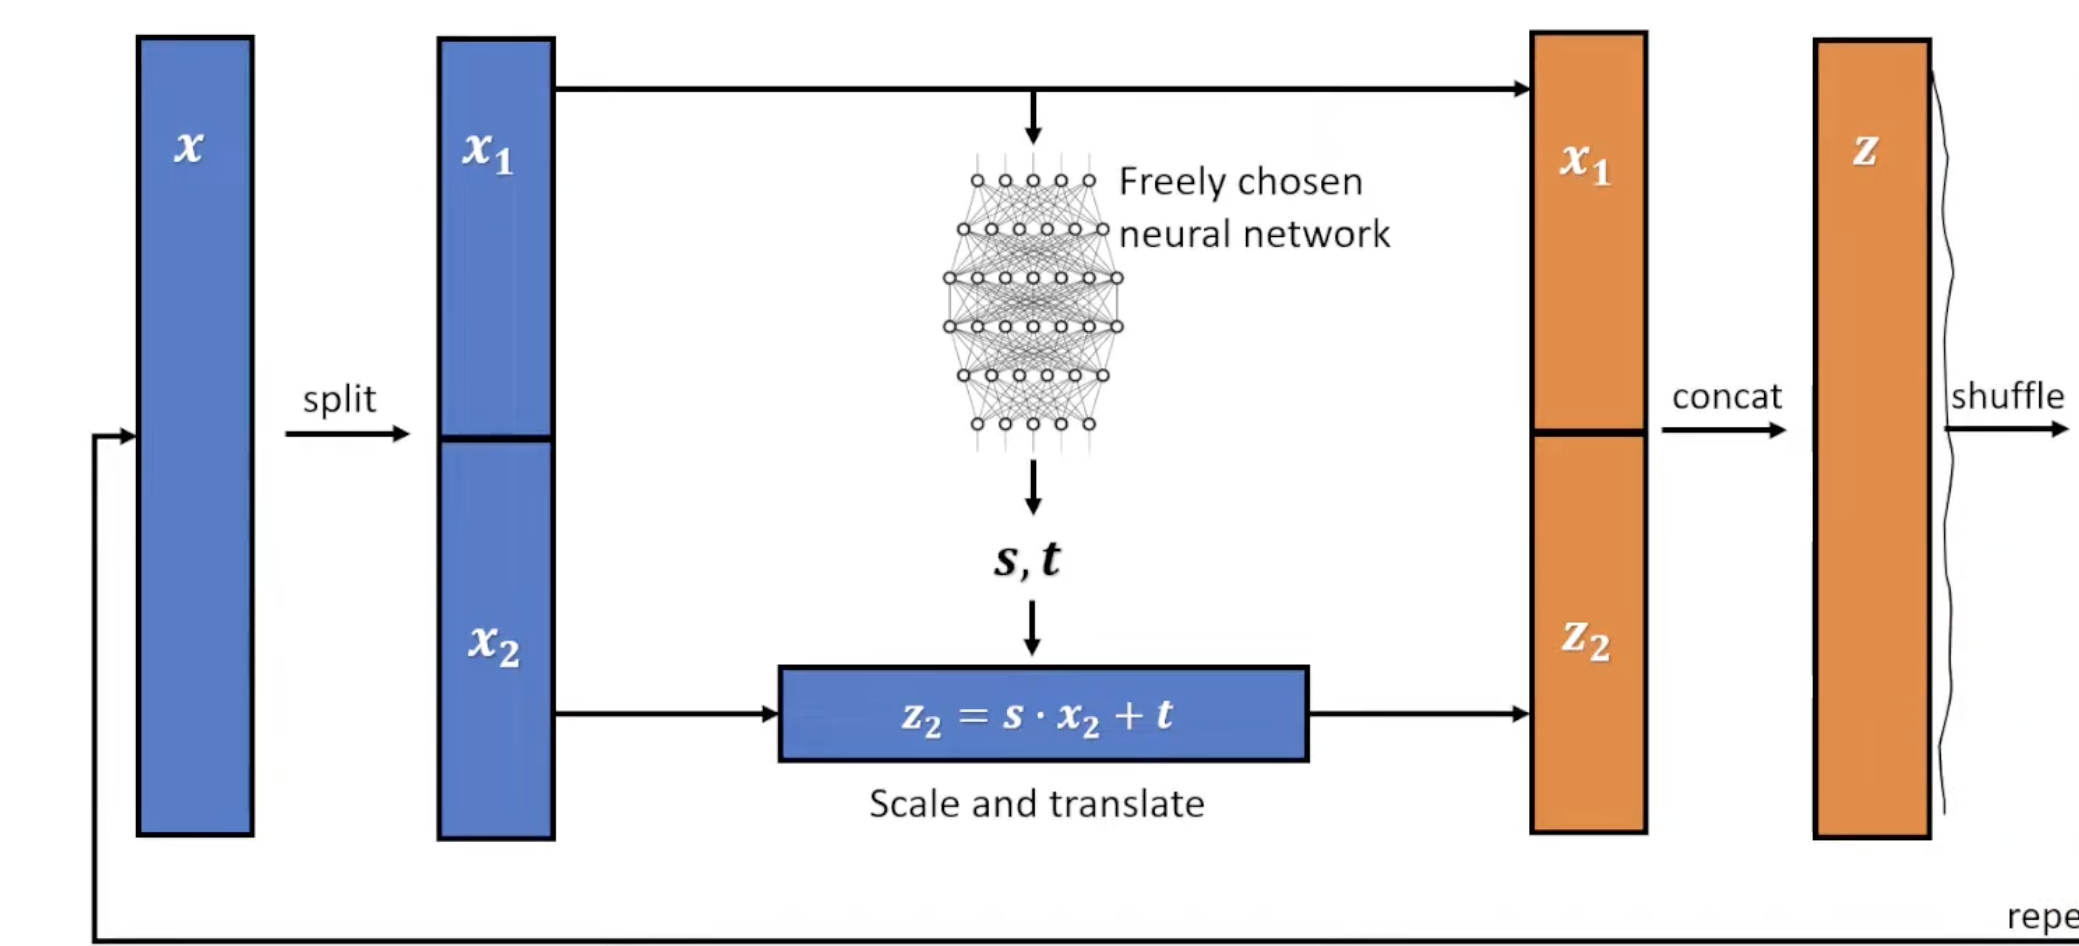
\includegraphics[width=0.7\textwidth]{normalizing-flows/realnvp.png}
    \caption{RealNVP architecture.}
\end{figure}

\subsubsection{Inversion}
Note that all the operations we applied to the input are invertible: both scaling and translation are invertible, and the shuffling operation is also invertible if we keep in memory the permutation used. Therefore, the RealNVP architecture is invertible, and we can compute the inverse transformation by simply inverting the operations.
\begin{figure}[H]
    \centering
    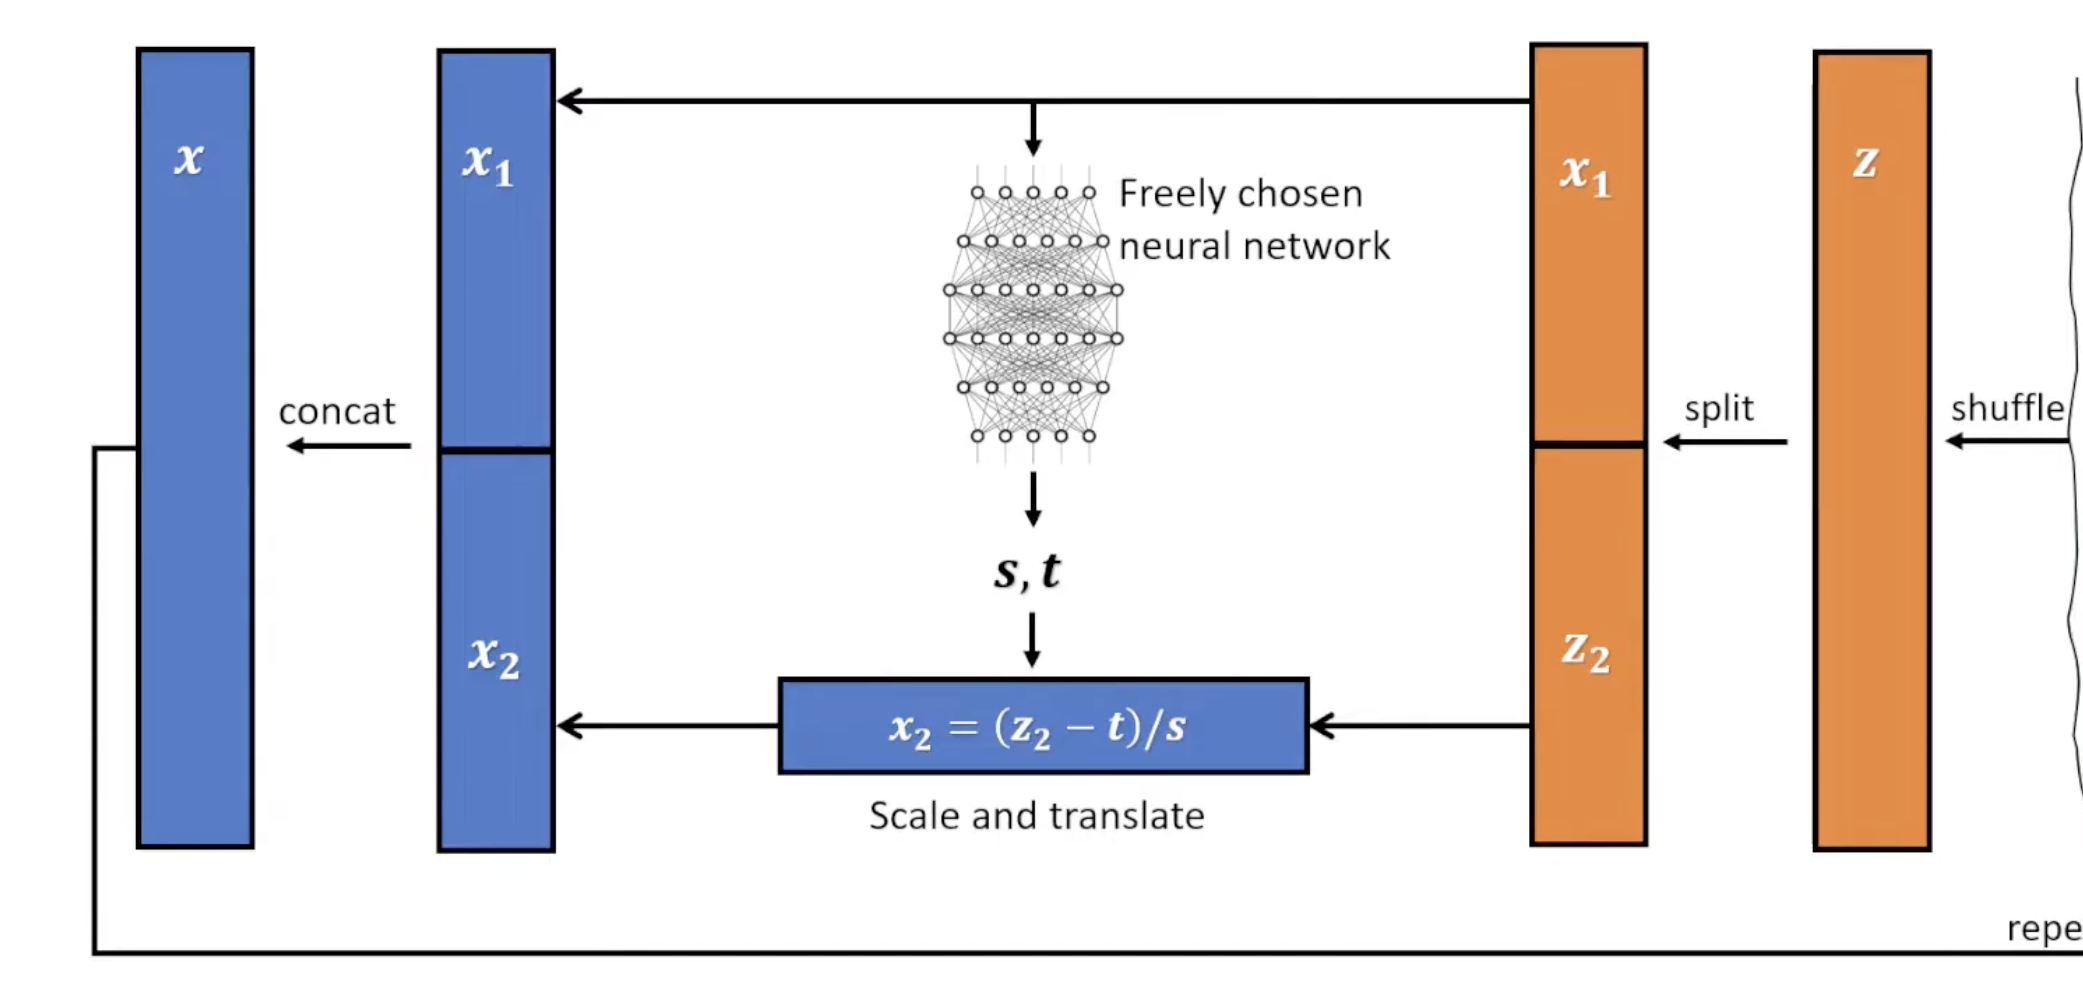
\includegraphics[width=0.7\textwidth]{normalizing-flows/realnvp-reverse.png}
    \caption{Reversing a coupling layer to form a decoder.}
\end{figure}
Explicitely, we can recover the input $x$ from the output $y$ by computing:
\begin{equation*}
    \begin{aligned}
        x_{1:d} &= y_{1:d}\\
        x_{d+1:D} &= (y_{d+1:D}-t(y_{1:d})) \odot \exp(-s(y_{1:d}))
    \end{aligned}
\end{equation*}

\subsection{Loss function}
To choose a loss function for the training of normalizing flows, we want to maximize the likelihood of the data under the model, that is to compute:
\begin{equation*}
    \argmax_{\theta} \log p_\theta(x) = \argmax_{\theta} \sum_{i=1}^n \log p_\theta(x_i)
\end{equation*}
In the case of normalizing flows, we can compute the likelihood exactly. Given a sample $x$ and a prior distribution over the latent space $p(z)$, we can compute $f(x)=z$ through the invertible learned function $f$. The evidence $p(x)$ can be computed using the change of variable formula:
\begin{equation*}
    p(x) = p(z)\cdot\left|\det\left(\frac{\dd z}{\dd x}\right)\right| = p(f(x))\cdot\left|\det J_f(x)\right|
\end{equation*}
where $J_f(x)$ is the Jacobian of the transformation $f$ at $x$. 

Therefore, we can traing the normalizing flow by optimizing:
\begin{equation*}
    \max_\theta\sum_{i=1}^n \log p_\theta(x_i) = \max_\theta\sum_{i=1}^n \left(\log p_\theta(f(x_i)) + \log\left|\det J_f(x_i)\right|\right)
\end{equation*}

In the case of RealNVP, the Jacobian of one coupling layer is:
\begin{equation*}
    J_f(x) = \partfrac{y}{x} = \begin{bmatrix}
        I_d & 0_{d, D-d}\\
        \partfrac{y_{d+1:D}}{x_{1:d}} & \diag\left(\exp(s(x_{1:d}))\right)
    \end{bmatrix}
\end{equation*}
The logarithm of the determinant of this matrix can be computed as:
\begin{equation*}
    \log\left|\det J_f(x)\right| = \log\prod_{j=1}^{D-d}\exp\left[s(x_{1:d})\right]_j = \sum_{j=1}^{D-d} \left[s(x_{1:d})\right]_j
\end{equation*}

\subsection{Training process}

\subsection{Example}

